\let\negmedspace\undefined
\let\negthickspace\undefined
\documentclass[journal]{IEEEtran}
\usepackage[a5paper, margin=10mm, onecolumn]{geometry}
%\usepackage{lmodern} 
\usepackage{tfrupee} 

\setlength{\headheight}{1cm} 
\setlength{\headsep}{0mm}     

\usepackage{gvv-book}
\usepackage{gvv}
\usepackage{cite}
\usepackage{amsmath,amssymb,amsfonts,amsthm}
\usepackage{algorithmic}
\usepackage{graphicx}
\usepackage{textcomp}
\usepackage{xcolor}
\usepackage{txfonts}
\usepackage{listings}
\usepackage{enumitem}
\usepackage{mathtools}
\usepackage{gensymb}
\usepackage{comment}
\usepackage[breaklinks=true]{hyperref}
\usepackage{tkz-euclide} 
\usepackage{listings}                                        
\def\inputGnumericTable{}                                 
\usepackage[latin1]{inputenc}                                
\usepackage{color}                                            
\usepackage{array}                                            
\usepackage{longtable}                                       
\usepackage{calc}                                             
\usepackage{multirow}                                         
\usepackage{hhline}                                           
\usepackage{ifthen}                                           
\usepackage{lscape}

\begin{document}

\bibliographystyle{IEEEtran}
\vspace{3cm}

\title{3.2.19}
\author{AI25BTECH11003 - Bhavesh Gaikwad}
{\let\newpage\relax\maketitle}

\renewcommand{\thefigure}{\theenumi}
\renewcommand{\thetable}{\theenumi}
\setlength{\intextsep}{10pt} 


\numberwithin{equation}{enumi}
\numberwithin{figure}{enumi}
\renewcommand{\thetable}{\theenumi}


\textbf{Question}: Two sides of a triangle are of lengths 5cm and 1.5cm. The length of the third side of the triangle cannot be\\
a) 3.6 cm\\
b) 4.1 cm\\
c) 3.8 cm\\
d) 3.4 cm\\

\textbf{Solution:}\\
Assume Triangle ABC with $\norm{\vec{AC}} = b = 1.5cm, \; \norm{\vec{AB}} = c = 5cm, \; \norm{\vec{BC}} = a$ \\
and Angle A = $\alpha$\\
Let $\vec{A} = \myvec{ 0 \\ 0}$\\
Therefore, $\vec{C} = \myvec{b \\ 0} = \myvec{ 1.5 \\ 0}$ and $\vec{B} = \myvec{c\cos\alpha \\ c\sin\alpha} = \myvec{5\cos\alpha \\ 5\sin\alpha}$\\\\


By Cosine Law,
\begin{equation}
a^2 = b^2 + c^2 - 2bc\cos\alpha
\end{equation}

\begin{align}
a^2 = 27.25 - 15\cos\alpha
\end{align}

\begin{equation}
\cos\alpha = \frac{27.25 - a^2}{15}
\end{equation}

\newpage

Option (A) a = 3.6cm
\begin{equation}
    \cos\alpha = \dfrac{27.25 - 12.96}{15} = \dfrac{14.29}{15}
\end{equation}

 \begin{equation}
\Rightarrow \, \alpha = 17.7^\circ     
 \end{equation}

\begin{figure}[htbp]
    \centering
    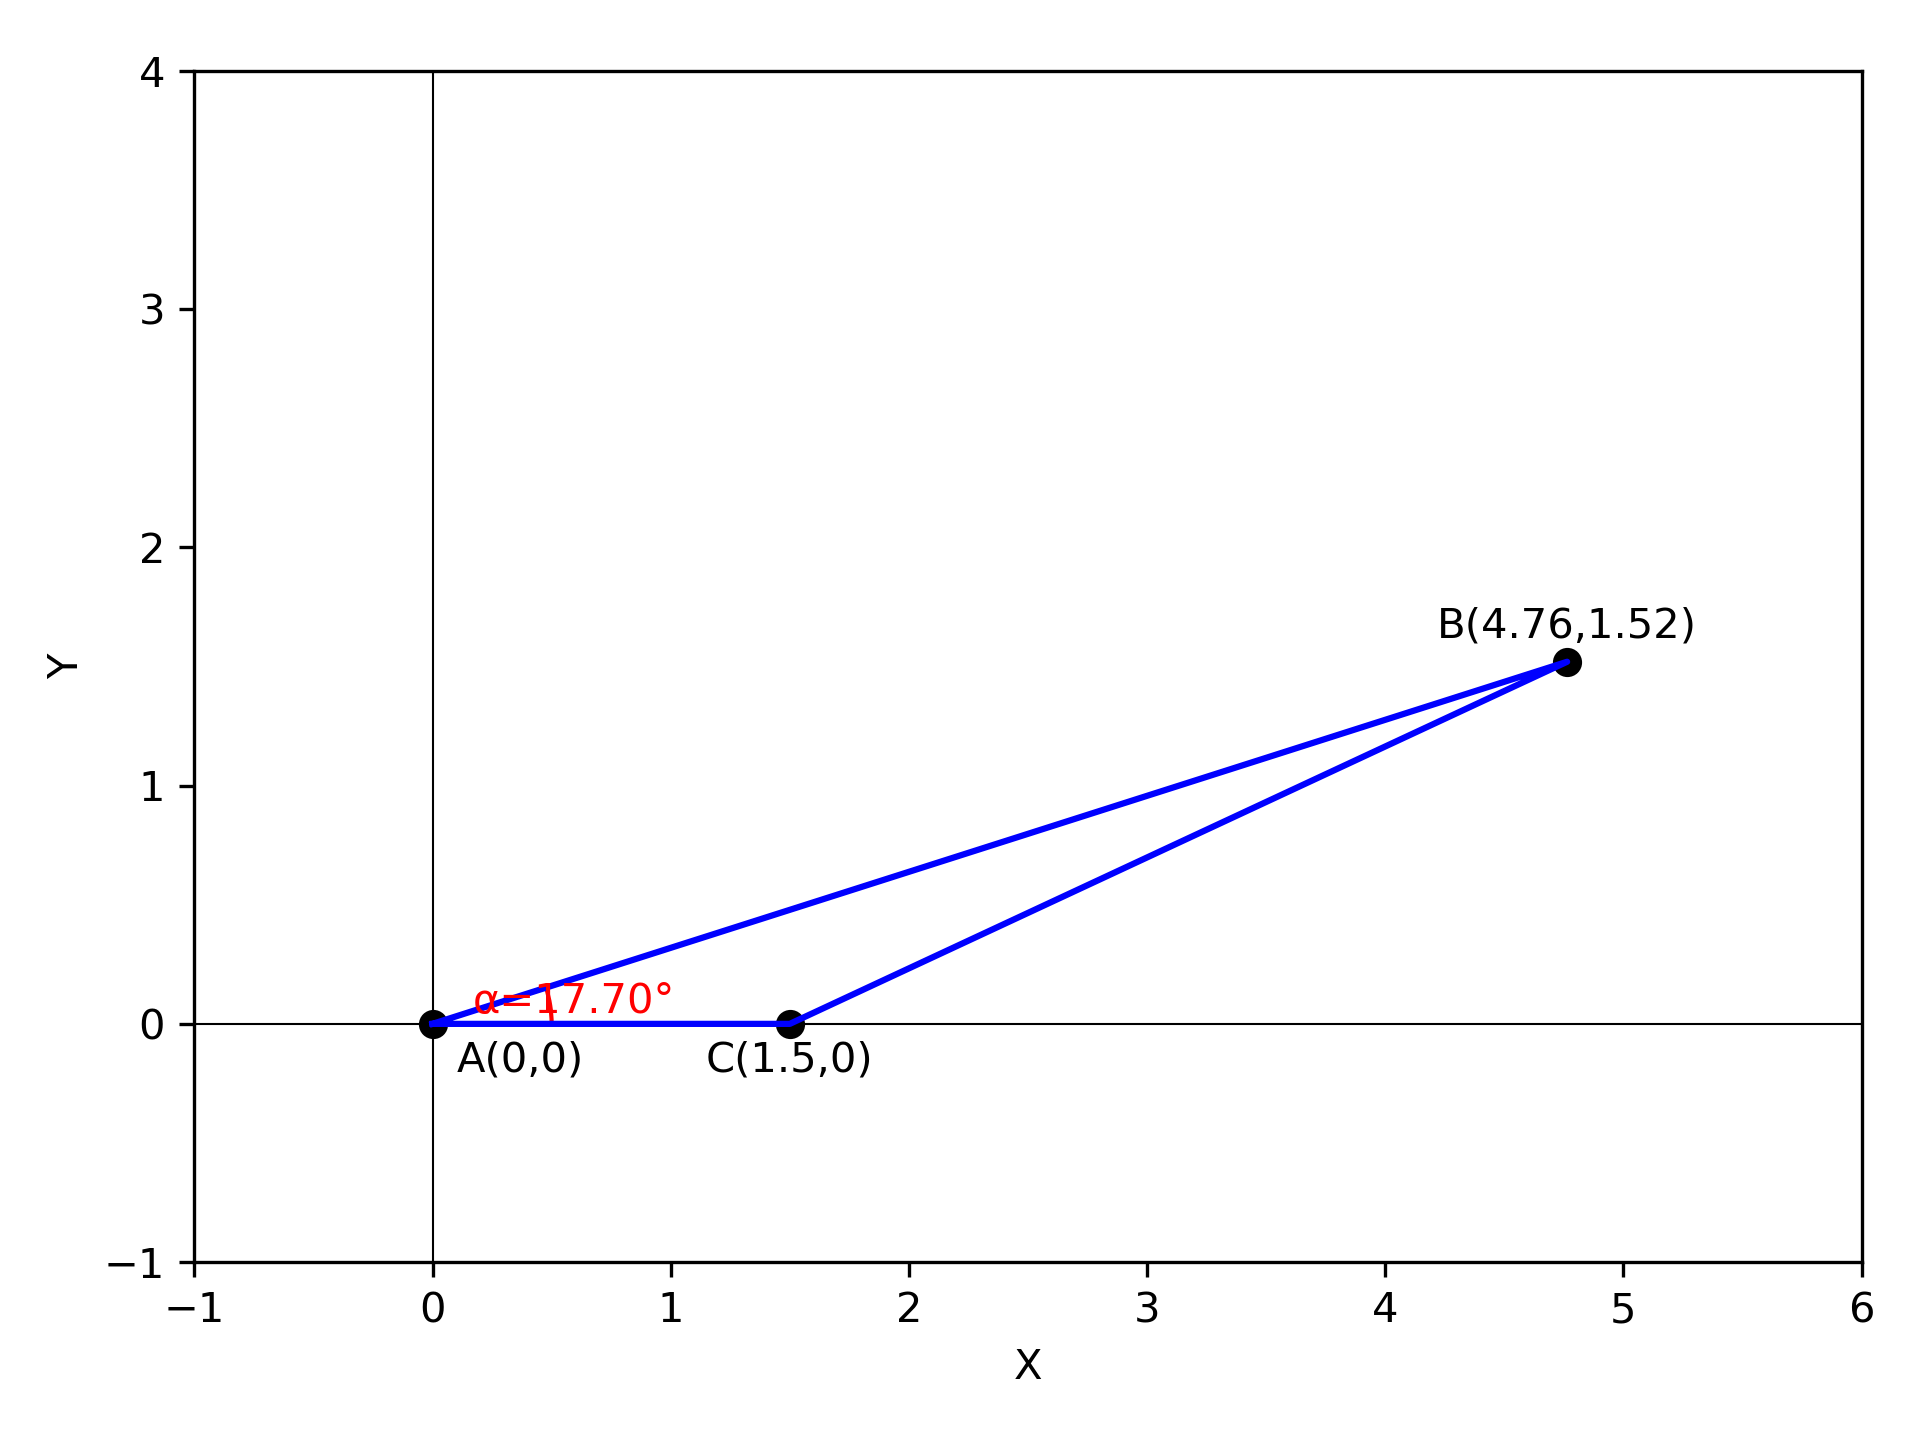
\includegraphics[width=\columnwidth]{figs/fig1.png}
    \caption{Triangle ABC of Option (A)}
    \label{fig:placeholder}
\end{figure}

\newpage

Option (B) a = 4.1cm
\begin{equation}
    \cos\alpha = \dfrac{27.25 - 16.81}{15} = \dfrac{10.44}{15}
\end{equation}

 \begin{equation}
\Rightarrow \, \alpha = 45.89^\circ     
 \end{equation}

\begin{figure}[htbp]
    \centering
    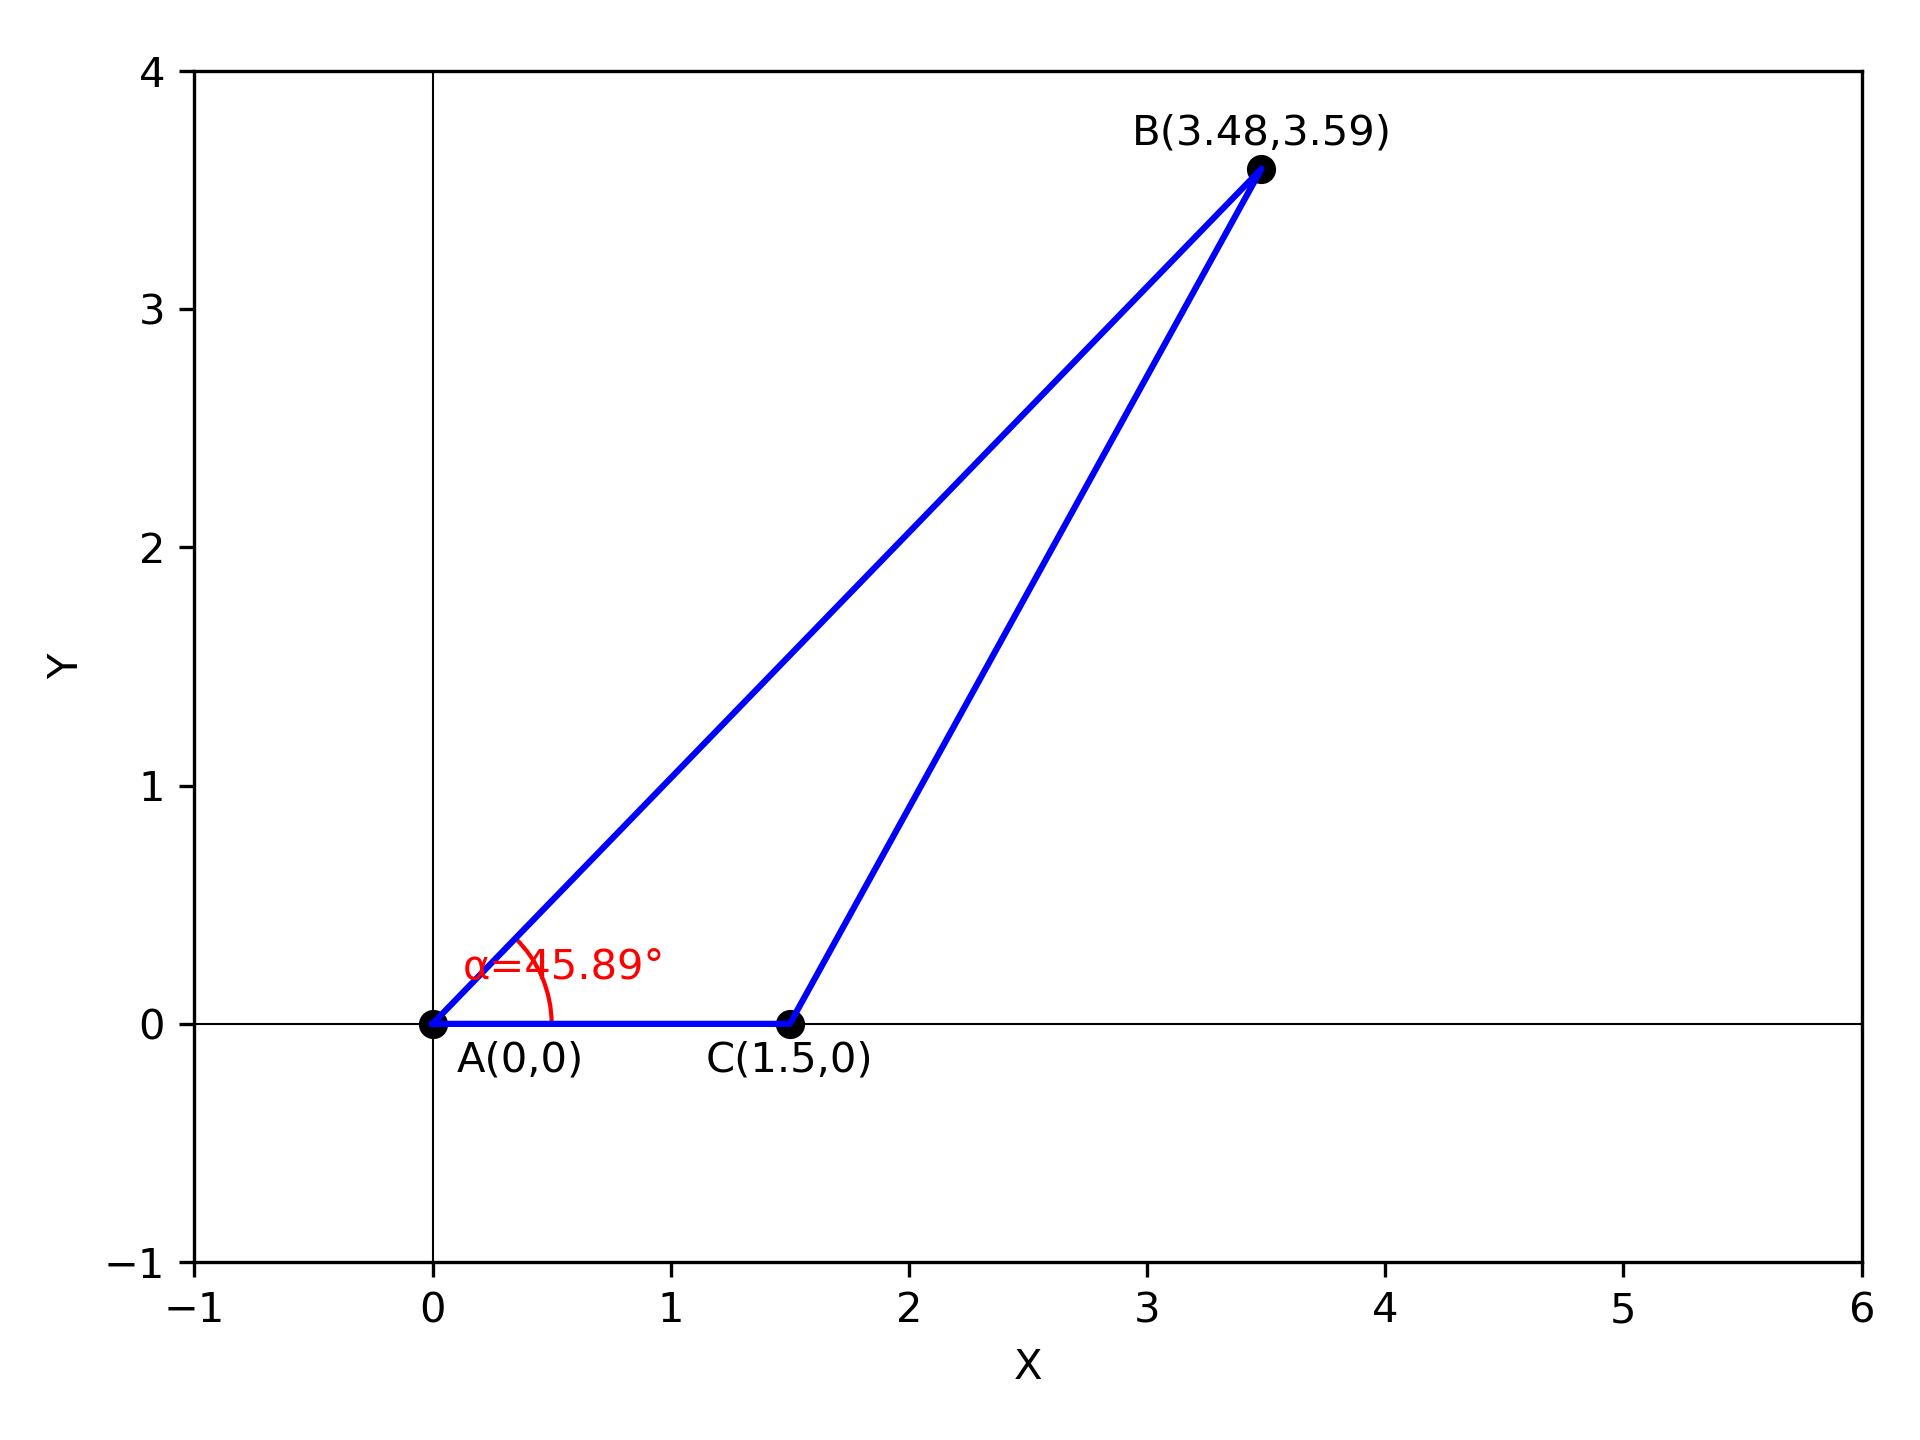
\includegraphics[width=\columnwidth]{figs/fig2.png}
    \caption{Triangle ABC of Option (B)}
    \label{fig:placeholder}
\end{figure}

\newpage

Option (C) a = 3.8cm
\begin{equation}
    \cos\alpha = \dfrac{27.25 - 14.44}{15} = \dfrac{12.81}{15}
\end{equation}

 \begin{equation}
\Rightarrow \, \alpha = 31.35^\circ     
 \end{equation}

\begin{figure}[htbp]
    \centering
    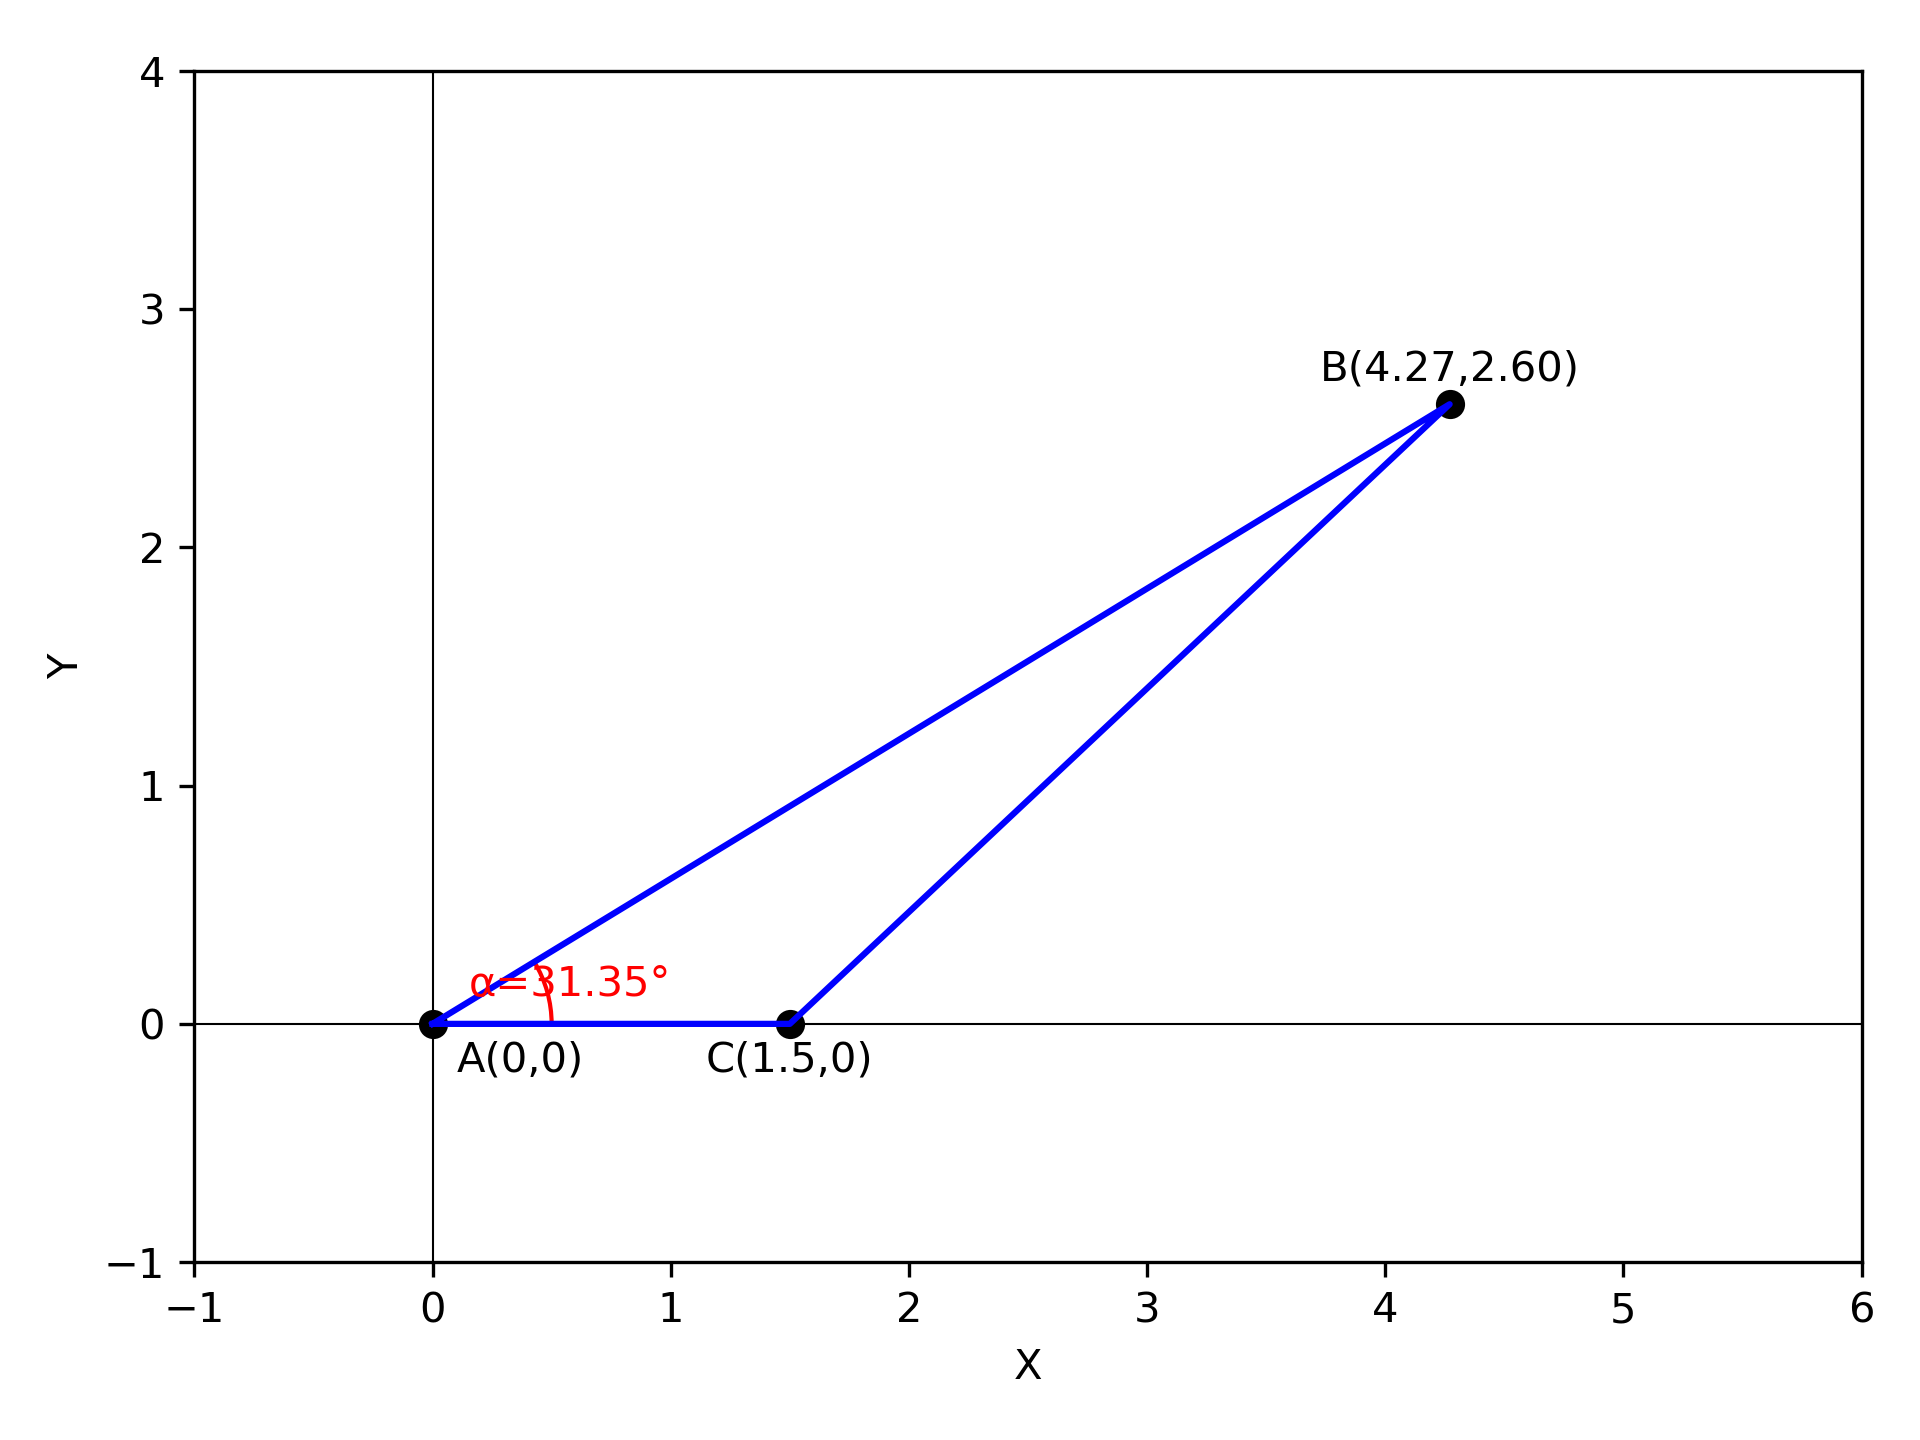
\includegraphics[width=\columnwidth]{figs/fig3.png}
    \caption{Triangle ABC of Option (C)}
    \label{fig:placeholder}
\end{figure}

\newpage

Option (D) a = 3.4cm
\begin{equation}
    \cos\alpha = \dfrac{27.25 - 11.56}{15} = \dfrac{15.69}{15}
\end{equation}
\begin{equation}
    \text{Here, } \cos\alpha > 1 \text{ which is not possible}
\end{equation}

\begin{align*}
    \boxed{\text{Thus, Option (D) is incorrect.}}
\end{align*}

\begin{figure}[htbp]
    \centering
    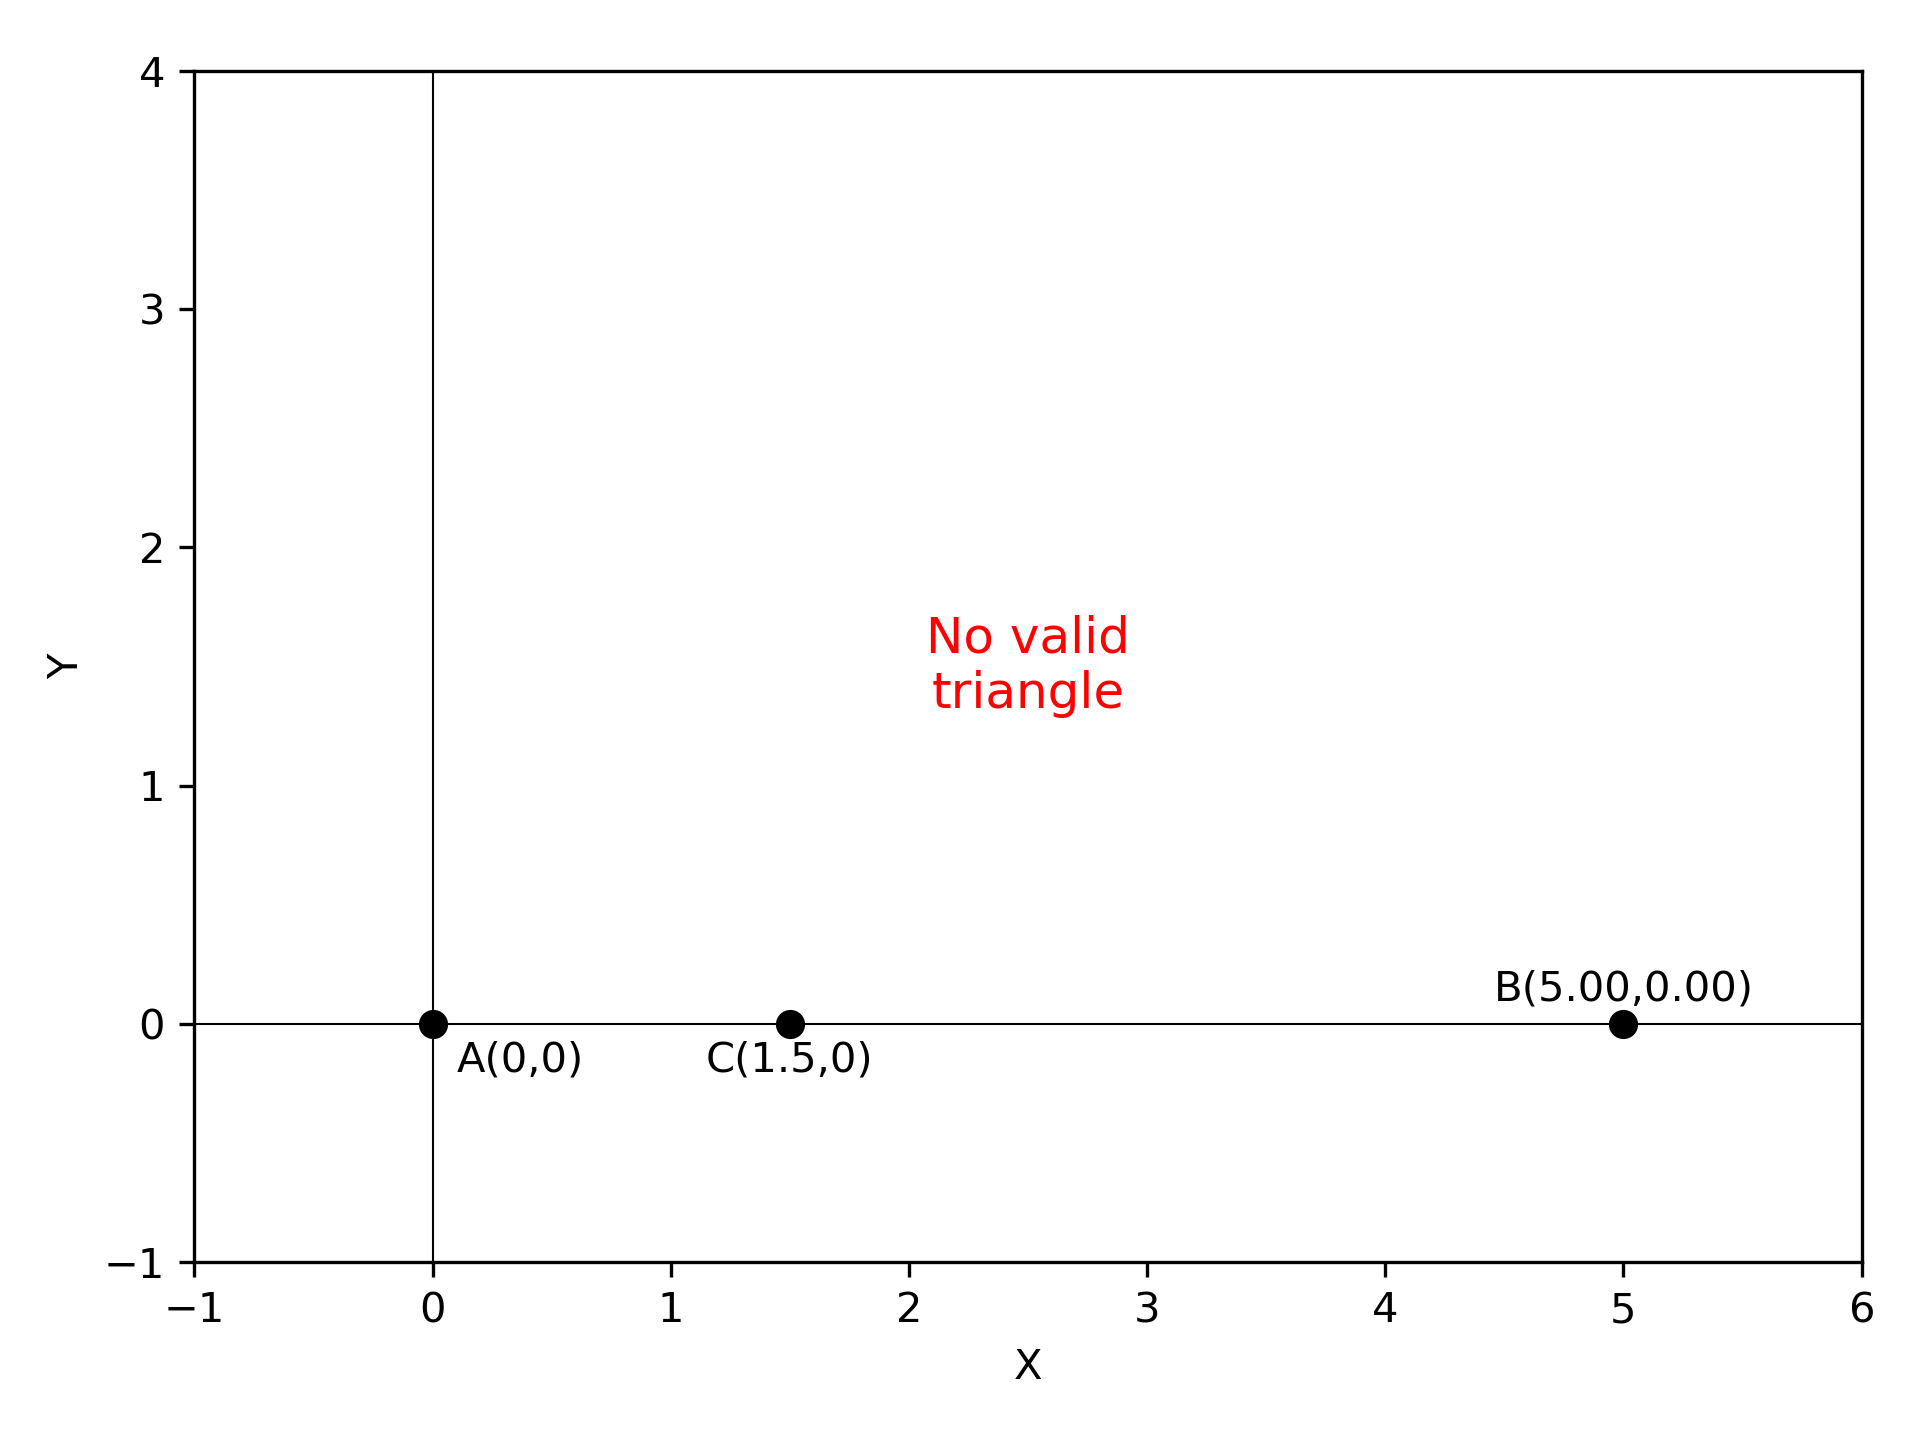
\includegraphics[width=\columnwidth]{figs/fig4.png}
    \caption{Image of Option (D)}
    \label{fig:placeholder}
\end{figure}

\end{document}  
